\documentclass{thesisreport}
\usepackage{todonotes}
\usepackage{parskip}
\usepackage{graphicx}
\usepackage{float}
\usepackage{multicol} %aggiunto da me
\usepackage{enumitem}


\begin{document}

 \thispagestyle{empty}

\def\lskip{\vspace{0.5cm}}


\begin{tabular}{p{7cm}p{10cm}}
ÉCOLE CENTRALE DE NANTES
&
\raggedleft UNIVERSITÀ DEGLI STUDI DI GENOVA	% for EMARO students
\end{tabular}

\vspace{2cm}

% EMARO students
\begin{center} \large\sc MASTER ERASMUS MUNDUS \\ \normalsize{EMARO+ ``European Master in Advanced Robotics''} \end{center}


\begin{center}
	2018 / 2019\\
	\lskip
	Master Thesis Report
	\lskip
	
	Presented by \lskip 
	
	Tommaso Elia \lskip
	
	28/12/2018 \lskip\lskip
	
	{\Large \textbf{Dialogue-based interaction processes with smart homes and companion robots}}
	
	\vfill

Jury \lskip
		
	\end{center}
	


\begin{tabular}{p{3cm}p{6cm}p{6cm} }
 President: & Name & Position (Institution) \\ & & \\ 
 Evaluators: & Name & Position (Institution) \\
	      & Name & Position (Institution) \\ 
	      & Name & Position (Institution) \\ & & \\  & & \\ 
  Supervisor(s):  & Fulvio Mastrogiovanni & Assistant Professor (UNIGE)\\
		  & Enrico Reboscio & Project Menager (DotVocal S.r.l.) \\
		  & Renato Zaccaria & Assistant Professor (UNIGE) \\
(EMARO)  & Co-supervisor from M1 & Position, M1 institution 
\end{tabular}

\lskip

\begin{flushleft}
 Laboratory: Laboratoire des Sciences du Numérique de Nantes LS2N
\end{flushleft}

\newpage
\thispagestyle{empty}
\null
\newpage
\addtocounter{page}{-1}
\pagestyle{fancy}
  
 
  \section*{Abstract}
   
 Do not forget to check each reference while importing in your Bibtex file.
 Especially, IEEExplore export may lead to ill-formatted conference name like \emph{Robotics and Automation, 
 IEEE International Conference on}.
 
 \newpage
 
 %\section*{Acknowledgements}
 %\newpage
 
\section*{Notations}
 
 \newpage
 
 \section*{Abbreviation}
 
 \begin{tabular}{p{2cm}p{12cm}}
 ADL & Activities of Daily Living\\
 AAL & Ambient Assisted Living \\
 IADL & Instrumental Activities of Daily Living \\
 DS & Dempster - Shafer \\
 DL & Description Logic \\
 SWRL & Semantic Web Rule Language\\
 OWL & Ontology Web Language\\
 EMS & Emergency Medical Services \\
 \end{tabular}
 
 \newpage
 
 \listoffigures
 
 \listoftables
 
 \tableofcontents
 
 
 \chapter*{Introduction}
 \addcontentsline{toc}{chapter}{Introduction}	 % non-numbered chapters do not appear in table of contents by default
 \section*{Background}
 The growth of the population with progress of medical techniques involve an increase in the number of elderly. Indeed in most of the industrialized countries the demographic and social trends lead to greater elderly among the population. The effects of the trends can be critical for emergency medical services, public and private health care and the individuals themselves. 
 The raising of the average age of the population mean an higher number of chronic diseases and therefore also emergency situations. 
 In the district of Kaiserslautern, Germany, a significant study was conducted showing that 44\% of Emergency Medical Services (EMS) are dedicated to elderly above 70 years of age.
 	\begin{figure}[H]
		\centering
		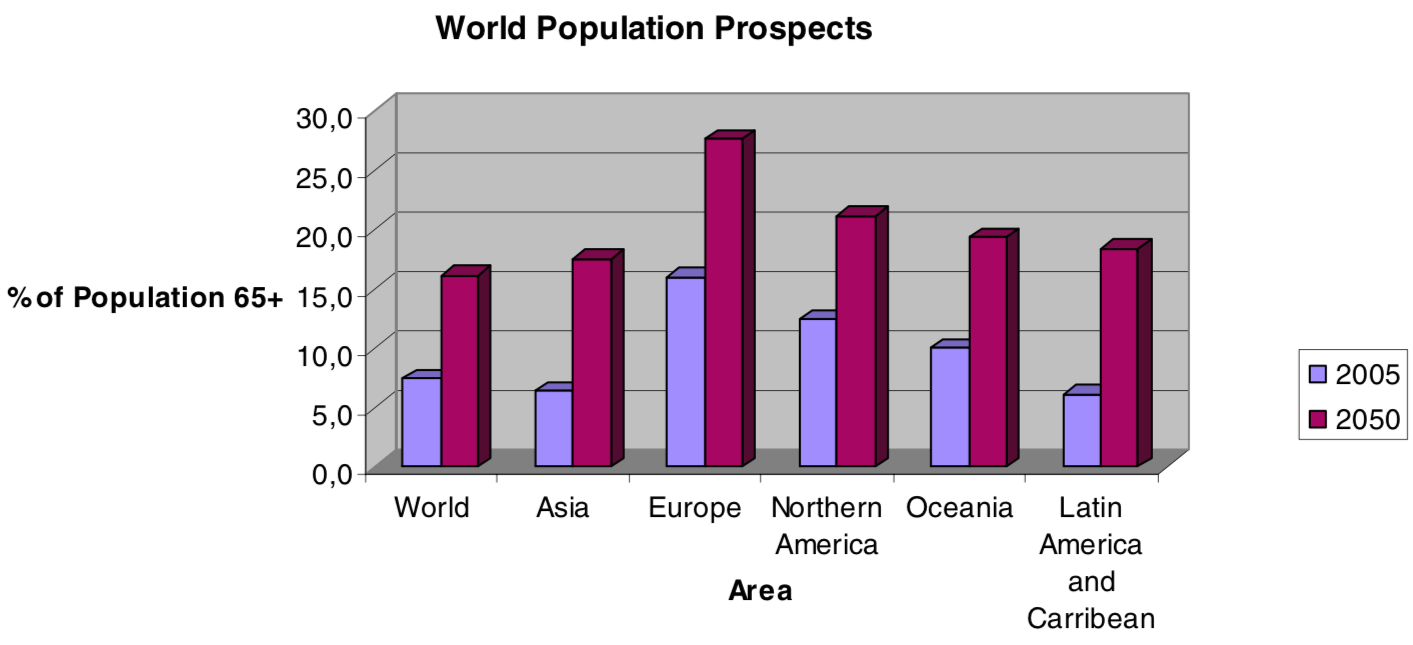
\includegraphics[width=12cm]{Thesis/data/populationProspect.png}
		\caption{\small{Demographical Change according to the United Nations World Population Prospects \cite{kleinberger2007ambient}}}
		\label{fig:populationProspect}
	\end{figure}
 Such a result lead to suppose, decline in service quality or an increase in the cost for such services or both. 
 
 \parskip  \parskip
 
 The Ambient Intelligence technologies help to cope with trends, providing proactive and conscious assistance and supporting the autonomy of the elderly. Indeed Assisted Living solutions, not only can they reduce the costs of managing and monitoring older people but they can also offer better \textit{quality of life} \cite{kleinberger2007ambient}. 
 
 \parskip \parskip
 
 To do this, so to guarantee an improved quality of life it is necessary ensure that the so-colled Activities of Daily Living (ADL) are correctly and regularly performed by the assisted \cite{buoncompagni2017towards}.. 
 
 As defined \cite{buoncompagni2017towards}, ADL are daily activities related to motion, rest, nutrition, and personal hygiene, which are a qualitative indicator of a person’s wellbeing, determine their quality of life and level of independence. 
 
 An architecture able to monitoring these kind of activities can provide very useful information about human behaviour to Human-Robot interaction o cooperation in smart environments \cite{bruno2014public}.  
 
 In literature it is possible distinguish two different approaches of monitoring: one is based on heterogeneous sensor distributed in an area used to deduce the state of the person inside a context \cite{aggarwal2011human}; the other achieve the information from wearable sensing so sensors located on the person body and able to detect the movements of the person \cite{bao2004activity}. 
 Therefore we can differentiate two different pivotal concepts:
 \begin{itemize}
    \item to monitor complex sequences of activities reported over time and detected by the interaction with various objects in the monitored area, smart environments are the favourite approach \cite{scalmato2012describing}.
    \item with the advent of the Inertial Measurement Unit (IMU) and therefore easily monitoring the acceleration and orientation of the limbs , the wearable sensing systems, which also be able to monitor bio signals, are without a doubt the preferred solution to monitor either body gestures or vital signs \cite{bruno2013analysis}.
\end{itemize}
 
Both these approaches are obviously very useful to detect the state of health of the monitored person and one does not exclude the others. 

\subsection*{ADL}
Our everyday activities tell us a lot about who we are and to ensure a certain level of independence \cite{buoncompagni2017towards}. For this reason at first it is very important to define them. 
\\
As early as late 1950s, we began to study the psychological, social and biological aspects of aging, analyzing the correlation between human actions and cognitive and motor capabilities \cite{buoncompagni2017towards}. 
\\

From \cite{Multidisciplinary} we can find the Index of activities of Daily Living where show a classification of the functional status of elderly people on the basis of their capability in the execution of 6 different activities in other words called ADLs \cite{buoncompagni2017towards}:
\begin{enumerate}[noitemsep,topsep=1pt,parsep=1pt,partopsep=1pt]
    \item \textit{bathing}
    \item \textit{dressing}
    \item \textit{toileting}
    \item \textit{transferring}
    \item \textit{continence}
    \item \textit{feeding}
\end{enumerate}

But these number of ADLs was then extended adding activities deemed relevant for the well-being of a person. These other nine activities, that take the name of Scale of Instrumental ADL \cite{lawton1970assessment} (IADL), require sufficient capabilities of social skills and planning capabilities using and interacting with everyday objects \cite{buoncompagni2017towards}:
\begin{enumerate}[noitemsep,topsep=1pt,parsep=1pt,partopsep=1pt]
    \item \textit{placing a telephone call}
    \item \textit{shopping}
    \item \textit{preparing food}
    \item \textit{housekeeping}
    \item \textit{doing the laundry}
    \item \textit{moving outdoor with public transports}
    \item \textit{moving indoor on foot}
    \item \textit{taking medications}
    \item \textit{handling finances}
\end{enumerate}
Nowadays, as explained in \cite{bruno2014public} the scale of IADL and the index of ADL are the \textit{de facto} standard indexes to evaluate person’s functional status\cite{buoncompagni2017towards}. 

In this essay the term ADL will assume a more general meaning, representing any  considered daily activities. 

\subsection*{Human Activity Recognition}
There are a lot documentations in literature where we discuss of the automatic recognition of ADL. There are often differences about adopted sensing equipment or in the choice of the type of sensors. But typically all the solution share a common paradigm: "\textit{distributed sensing, centralized reasoning}". The sensor information are distributed as raw data, with minimal or no processing, and made available to the reasoning system responsible for analyzing them to extract high level information, the ADLs.   

Tanti articoli in letteruatura parlano del riconoscimento di ADL,
Differenze nei dispositivi di rilevamaento, nella scelta dei sensori e nella tecnica per la laro analisi.  
Quasi tutte le soluzioni presentano però un paradigma, sensing distribuito e ragionamento centralizzato. Questo significa che i dati sensoriali sono dati grezzi, con una minima o nessuna elaborazione, sono resi disponiibili al "ragionatore" responsabile dell'anilisi di questi per estrarre informazioni di alto livello ovverto le ADL. 
Una possibile soluzione è usare un gran numero di sensori binari per la loro facile interpretazione (es: interruttore della luce ON/OFF) ed il loro basso costo. Le inforamzioni sensoriali devono però essere organizzati e analizzati in strutture di più alto livello. Per fare ciò in letteratura, la soluzione più utilizzata e intelligente è farlo con le ontologie. 



Un grande corpus di letteratura tratta del riconoscimento automatico di ADL. Oltre alle differenze nelle apparecchiature di rilevamento adottate e, di conseguenza, nel middleware per la gestione dei dati sensoriali e nelle tecniche per la loro analisi, la maggior parte delle soluzioni seguono lo stesso principio di funzionamento del "sensing distribuito, ragionamento centralizzato". In questo paradigma, i dati sensoriali grezzi (eventualmente) eterogenei vengono raccolti e, con nessuna o minima pre-elaborazione, resi disponibili al sistema di ragionamento responsabile dell'analisi per estrarre informazioni di alto livello relative all'esecuzione di ADL. Ad esempio, la più ricca tra queste soluzioni utilizza un numero elevato di sensori binari economici (come i sensori di presenza per rilevare se c'è una persona in un'area, sensori aperti / chiusi per porte e finestre, sensori on / off per interruttori della luce, ecc.) e si basano su ontologie per l'estrazione di informazioni ad alto livello relative all'ADL da dati sensoriali [6] [26], senza elaborazione intermedia.

 
 
 \chapter{State of the art}
 
%  \section{First topic}
 
%  \section{Second topic}

%  \chapter{Actual work}
  
%  When dealing with rectangled triangles (see Figure \ref{triangle}) I sometimes used this theorem from \cite{pythm001}:
%  \begin{equation}\label{theo}
%   a^2 + b^2 = c^2
%  \end{equation}The demonstration is in Appendix \ref{sec:prooftheorem}.
 
%  \begin{figure}[h]\centering
%   \includegraphics[width=.5\linewidth]{triangle1}
%   \caption{A triangle with letters} \label{triangle}
%  \end{figure}
 
 
%  \chapter{Failed experiments}
 
%  When trying to draw a rectangled triangle, my program comes up with Figure \ref{triangle2} that is neither rectangled nor a triangle.
 
%   \begin{figure}[h]\centering
%   \includegraphics[width=.5\linewidth]{triangle2}
%   \caption{Triangle drawn by my program. Note the 4th side.} \label{triangle2}
%  \end{figure}
 
 
%  \chapter*{Conclusion}
%  \addcontentsline{toc}{chapter}{Conclusion}
 
 
 
%  % switch to A-B-C chaptering
%  \appendix	
 
%  \chapter{Proof of theorem \ref{theo}}
%  \label{sec:prooftheorem}
 
 
%  \begin{proof}
% \eqref{theo} was already demonstrated in \cite{euclides300}.
% \end{proof}
 
 \addcontentsline{toc}{chapter}{Bibliography}

 \bibliographystyle{IEEEtran}
 
 \bibliography{biblio}
 
 
 
 
\end{document}
